%In this section, we aim to better understand object memorability by focusing on visually manifesting factors that influence whether an object in an image is more memorable or forgettable to humans. \B{give an overview of these factors, e.g. color, saliency, size, etc.}%We first investigate the role that simple color features play in determining object memorability.


In this section, we aim to better understand how object memorability is influenced by visual factors that manifest themselves in natural images. Specifically, we study the relationship between simple color features, visual saliency, object semantics, and how memorable or forgettable an object in an image is to humans. The results of this study can be used to guide the development and innovation of automated algorithms that can predict object memorability.


\subsection{Can simple features explain memorability?}

\begin{figure}[!htb]
\centering
\subfigure{\centering \includegraphics[width=0.47\textwidth]{figures/results/simple_features/color_corrs.png}}
\vspace{-5mm}\caption{\footnotesize\textbf{Simple color features do not explain object memorability.} Correlations of object memorability scores with hue and saturation are near zero, and only value shows a very weak correlation.}\label{fig:simple}
\end{figure}

While simple low-level image features are traditionally poor
predictors of image memorability \cite{isola11} (with good reason
\cite{konkle10}), the question arises whether such features play any
role in determining object memorability in images. To address this
query and following a similar strategy as in \cite{isola11,isola14},
we compute the mean (and variance) of HSV color of each object in our
dataset, i.e. first and second order  statistics of pixel color within
an object's ground truth segmentation, and correlate it (Spearman rank
correlation) with the underlying object memorability score (refer to
Figure \ref{fig:simple}). We see that the mean ($\rho = 0.1$) and
variance ($\rho=0.25$) of the V channel show weak correlation with
object memorability, suggesting that brighter and higher contrast
objects may be more memorable. On the other hand, essentially no
relationship exists between memorability and either the H or S
channels. This slightly deviates from the findings in \cite{isola11},
which show mean hue to be weakly predictive of image
memorability. This difference could be due to the fact that many
images of the dataset in \cite{isola11} show blue and green outdoor
landscapes as being less memorable than warmly colored human faces and
indoor scenes, while our dataset contains plenty of indoor objects and
people and outdoor scene-related segments such as sky and ground are
not included as objects. From these results, we see that, like image
memorability, simple pixel statistics do not play a significant role
in determining object memorability in images.



\subsection{What is the role of saliency in memorability?}

Intuitively, the regions within an image that are most salient are likely to have a higher probability of being remembered, since they will draw the attention of viewers and a majority of a viewer’s eye fixations will be spent looking at those regions.. On the other hand, it is conceivable that some visually appealing regions will not be memorable, especially since aesthetic images are known to be less memorable \cite{isola11}, \cite{isola14}. When can visual saliency predict object memorability and what are the possible differences between these two phenomena? Quantifying the precise relationship between saliency and memorability will be paramount  towards understanding object memorability in greater depth.

To this aim, we utilized the eye fixation dataset made available for the Pascal-S dataset in \cite{yin14}. With this dataset in hand, we first calculated the number of unique fixation points within the area of each object and computed the correlation between this metric and the object’s memorability score (Figure \ref{fig:scatterFixation} a). We found this correlation to be positive and considerably high ($\rho = 0.71$), suggesting that fixation count and visual saliency may drive object memorability considerably. However, the large concentration of points on the bottom left part of scatter plot in Figure \ref{fig:scatterFixation} a suggests that part of the reason for this high correlation is that objects that have not been viewed at all have essentially no memorability. Indeed, only objects that have been seen can be remembered. In addition, the points toward the top left appear to decrease in trend. Looking deeper, Figure \ref{fig:fixCorr} plots the change in correlation between object memorability and fixations as the minimum number of fixations inside objects increases. The downward monotonic trend indicates that as the number of fixations inside an object increases, the predictive ability diminishes significantly. In addition, Figure \ref{fig:fixCorr} plots the correlation between object memorability and number of fixations as a function of total number of objects in an image. Similar to the previous trend, as the number of objects in an image increases, the correlation between saliency i.e. number of fixations and memorability score decreases sharply. This finding is in agreement with the two remaining scatter plots in Figure \ref{fig:scatterFixation} b (shows that the memorability of an object decreases in the presence of many other objects) and Figure \ref{fig:scatterFixation} c (shows that number of fixations decreases with the number of objects). This makes intuitive sense since people have more to look at in an image when more objects are present, and so they may look less at any one object, especially if they compete for saliency, and therefore may have a more difficult time remembering those objects.

\begin{figure}[t]
\centering
\subfigure{\centering \includegraphics[width=0.5\textwidth]{figures/results/fixation/mem-fix-corr-by-factors.png}}
\vspace{-5mm}\caption{\footnotesize\textbf{Correlation between object memorability and number of fixations.} add-in later. }\label{fig:fixCorr}
\end{figure}

To sum up, saliency is a surprisingly good index of object memorability in simple contexts where there are few objects in the image, or when an object has few interesting points, but it is a much weaker predictor of object memorability in complex scenes containing multiple objects that have many points of interest (Figure \ref{fig:fixQual}).

\begin{figure}[b]
\centering
\subfigure{\centering \includegraphics[width=0.5\textwidth]{figures/results/fixation/fix_corr_set.png}}
\vspace{-5mm}\caption{\footnotesize\textbf{Correlation between object memorability and number of fixations.} add-in later. }\label{fig:scatterFixation}
\end{figure}

\textbf{Center Bias: } Figure \ref{fig:fixPos} elucidates another example where saliency and memorability diverge. Previous studies related to visual saliency have showed that saliency is heavily influenced by center bias \cite{judd09}, \cite{sun08}, primarily due to photographer bias (also evident from the leftmost plot in Figure \ref{fig:fixPos}) and viewing strategy \cite{tseng2009}. Since our data collection experiment tries to control for the viewing strategy, memorability exhibits comparatively less center bias than saliency. This is most apparent when considering the difference in the solid ellipse in the right plot (shows where $95\%$ of fixation positions are located), and the dashed ellipse (shows where the $95\%$ of the above-median memorable objects are located).

%Our work serves as the first direct evidence that saliency and memorability differ from each other by exploring the differences and overlap between the two.
%To the best of our knowledge, our work is the first to show the differences and overlap between saliency and memorability and how the two phenomena differ from each other.

\begin{figure}[t]
\centering
\subfigure{\centering \includegraphics[width=0.45\textwidth]{figures/results/fixation/positions_final.png}}
\vspace{-5mm}\caption{\footnotesize\textbf{Positions.} add-in later. }\label{fig:fixPos}
\end{figure}

\begin{figure}[t]
\centering
\subfigure{\centering \includegraphics[width=0.45\textwidth]{figures/results/fixation/qual/qual.png}}
\vspace{-5mm}\caption{\footnotesize\textbf{Saliency Fail cases.} add-in later. }\label{fig:fixQual}
\end{figure}


 \label{sec:fix}

\subsection{How do object categories affect memorability?}\label{sec:obLabel}

In the previous section, we explored the relationship between visual saliency of an object and its memorability. Now, we explore how an object's category influences the probability that it will be remembered.

\subsubsection{Are some object categories more memorable?}

For this analysis, we had three in-house annotators manually label the object segmentations in our dataset. The annotators were provided the original image (for reference) and the object segmentation and asked to assign a single category to the segment out of $7$ possible categories: animal, building, device, furniture, nature, person, and vehicle. We chose these categories so that a wide range of object classes could be covered. For example, category ``device” includes objects like utensils, bottles, and televisions, while ``nature” includes objects like trees, mountains, and flowers, and “vehicle” contains cars, bikes, and airplanes. Figure \ref{fig:avgMem} shows the distribution of the memorability scores of all $7$ object categories in our dataset.

\begin{figure}[!htb]
\centering
\subfigure{\centering \includegraphics[width=0.45\textwidth]{figures/results/obLabel/memScore_dist2.png}}
\vspace{-5mm}\caption{\footnotesize\textbf{Average memorability per object class.} Figure showing some object classes are more memorable than others. }\label{fig:avgMem}
\end{figure}

Results in Figure \ref{fig:avgMem} give a sense of how  memorability changes across different object categories. Animal, person, and vehicle are all highly memorable classes each associated with  an average memorability score greater than or close to $0.5$. Interestingly, all other categories have an average memorability lower than $0.25$, indicating that humans do not remember objects from these categories very well. In particular, furniture is the least memorable category with an average score of only $0.14$. This is possibly due to the fact that most objects in the furniture, nature, and building categories either appear mostly in the background or are occluded, which likely decreases their memorability significantly. In contrast, objects from the animal, person, and vehicle categories appear mostly in the foreground, leading to a higher memorability score on average. Interestingly, the most memorable objects from building, furniture, and nature tend to have an average memorability in the range of $0.4 - 0.8$, whereas the score of the most memorable objects from person, animal and vehicle is higher than $0.9$. %This is particularly interesting as these top objects are not occluded and most of them tend to appear in the foreground. 
While the differences in the memorability of different object categories could be driven due to factors like occlusion, size, background/foreground, or photographic bias, the distribution in Figure \ref{fig:avgMem} suggests that humans remember some object classes such as person, animal, and vehicle irrespective of external nuisance factors and these categories are \textit{intrinsically} more memorable than others.


%distribution of the most memorable objects within each class suggest that memorability could be an intrinsic property of an object class.  The right side of the figure presents an interesting analysis This analysis is particularly interesting as these top objects are not occluded and most of them tend to appear in the foreground. The top $20$ most memorable objects from person, animal and vehicle have memorability higher than $0.90$ whereas the average memorability of the top $20$ objects from building, furniture, and nature is lesser than $0.70$. While the differences in the memorability of different classes could be driven primarily due to factors like occlusion, size, background/foreground, the results in table \ref{tab:avgMem} suggest that memorability could be an intrinsic property of an object class and some object classes like person, animal, vehicle are in general intrinsically more memorable than classes like furniture, nature etc.
%



\subsubsection{Exploring category-specific memorability}


\begin{figure*}[!htb]
\centering
\subfigure{\centering 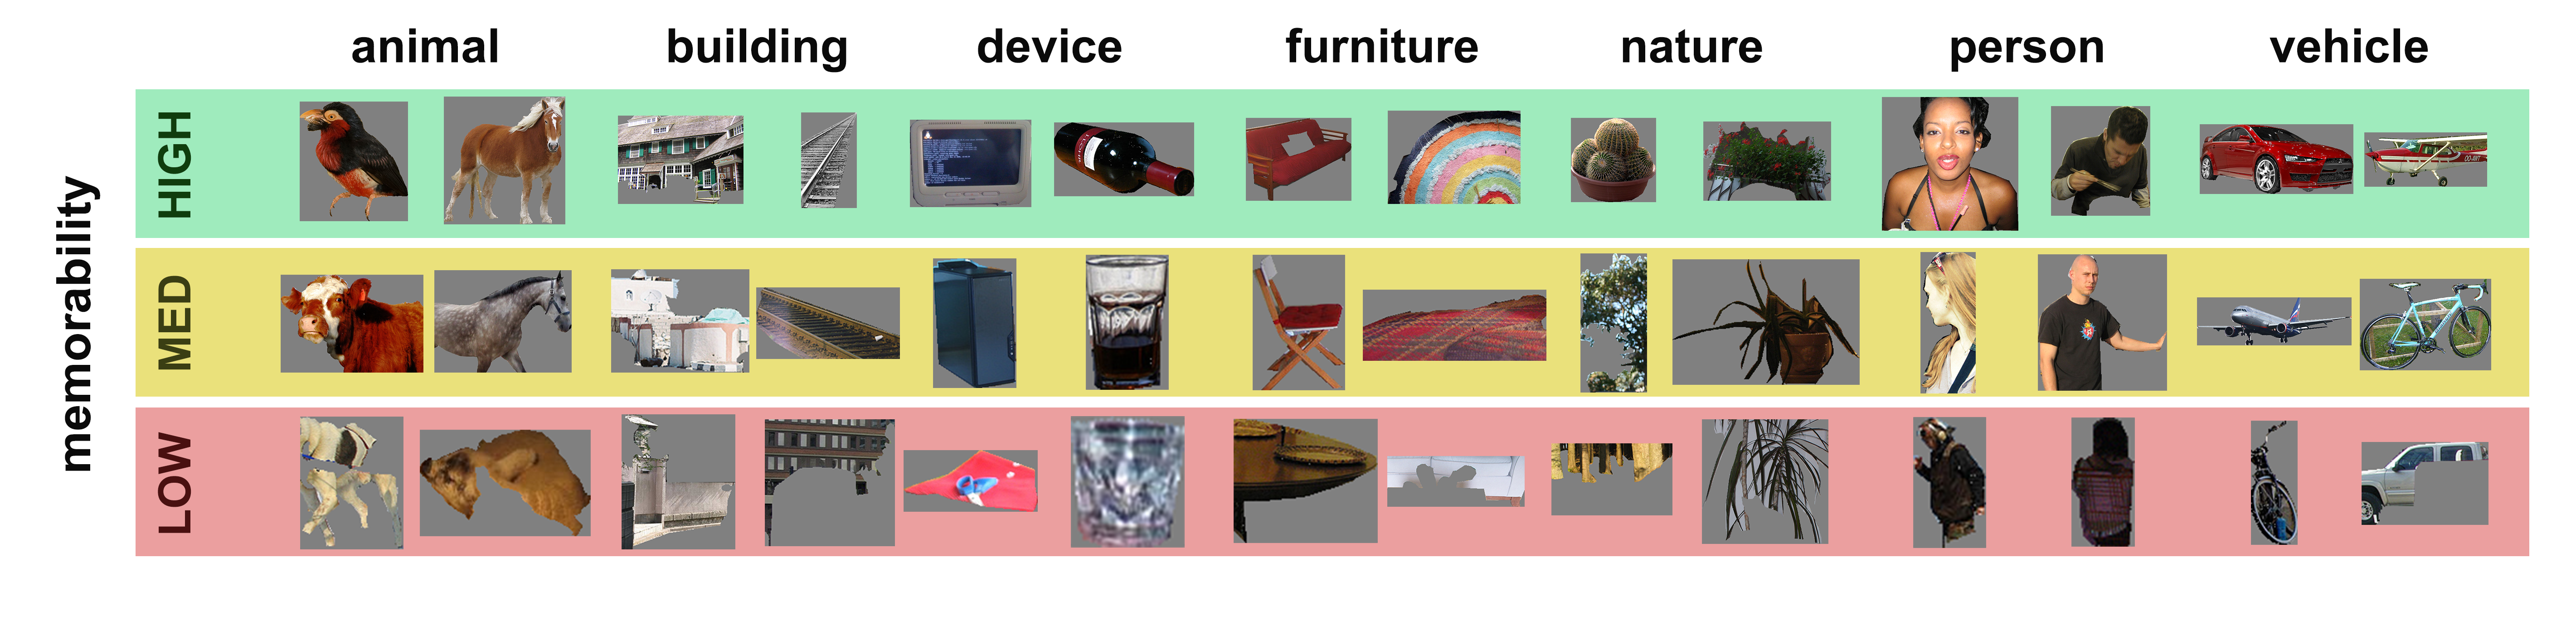
\includegraphics[width=1\textwidth]{figures/results/obLabel/qual_cat_v2.png}}
\vspace{-24pt}\caption{\footnotesize\textbf{Memorability of object categories.} Most memorable, medium memorable and least memorable objects from each of the $7$ categories.}\label{fig:obLabelQual}%\vspace{-12pt}
\end{figure*}

As demonstrated above, some object categories (i.e. animal, person, and vehicle) tend to be more memorable than others. However, not all objects in the same category are equally memorable. The examples in Figure \ref{fig:obLabelQual} show the most memorable, medium memorable, and least memorable objects for each category. Across categories, non-memorable objects tend to be those that are occluded and obstructed by other objects. What other category-related factors could influence the memorability of objects? Among the possible factors, we explore how category-specific object memorability is influenced by \textbf{(i)} the number of objects in an image and \textbf{(ii)} the presence of other object categories.


\vspace{3pt}\noindent\textbf{Number of objects:} %We first examined how the memorability of each object class is affected by the number of objects inside an image.
Figure \ref{fig:obLabelChange} shows the change in average memorability for the different categories when the minimum number of objects within an image is increased. Results indicate that the number of objects present in an image is an important factor in determining memorability. For example, as the number of objects in an image increases, the memorability of animals and vehicles decreases sharply, most likely as a result of competition for attention. Interestingly, the memorability of the person category does not change significantly when an increasing number of objects exist in the image. This suggests that people are not only one of the most memorable object categories, but that their memorability is the least sensitive to the presence of object clutter in an image. This may be because a single person steals most of the viewer's attention in an image, but how is this behavior characterized in the presence of other multiple people in the same image? To answer this, we turn to the question of interclass memorability next.

\begin{figure}[!t]
\centering
\subfigure{\centering \includegraphics[width=0.47\textwidth]{figures/results/obLabel/memScore_change2.png}}
\vspace{-5mm}\caption{\footnotesize\textbf{Object number affects category-specific memorability.} For each category, a curve is plotted that shows the change in average memorability with an increase in the number of objects. The memorability of objects belonging to categories like animals and vehicles goes down significantly with an increase in object number.}\label{fig:obLabelChange}
\end{figure}

\begin{figure}[!b]
\centering
\subfigure{\centering 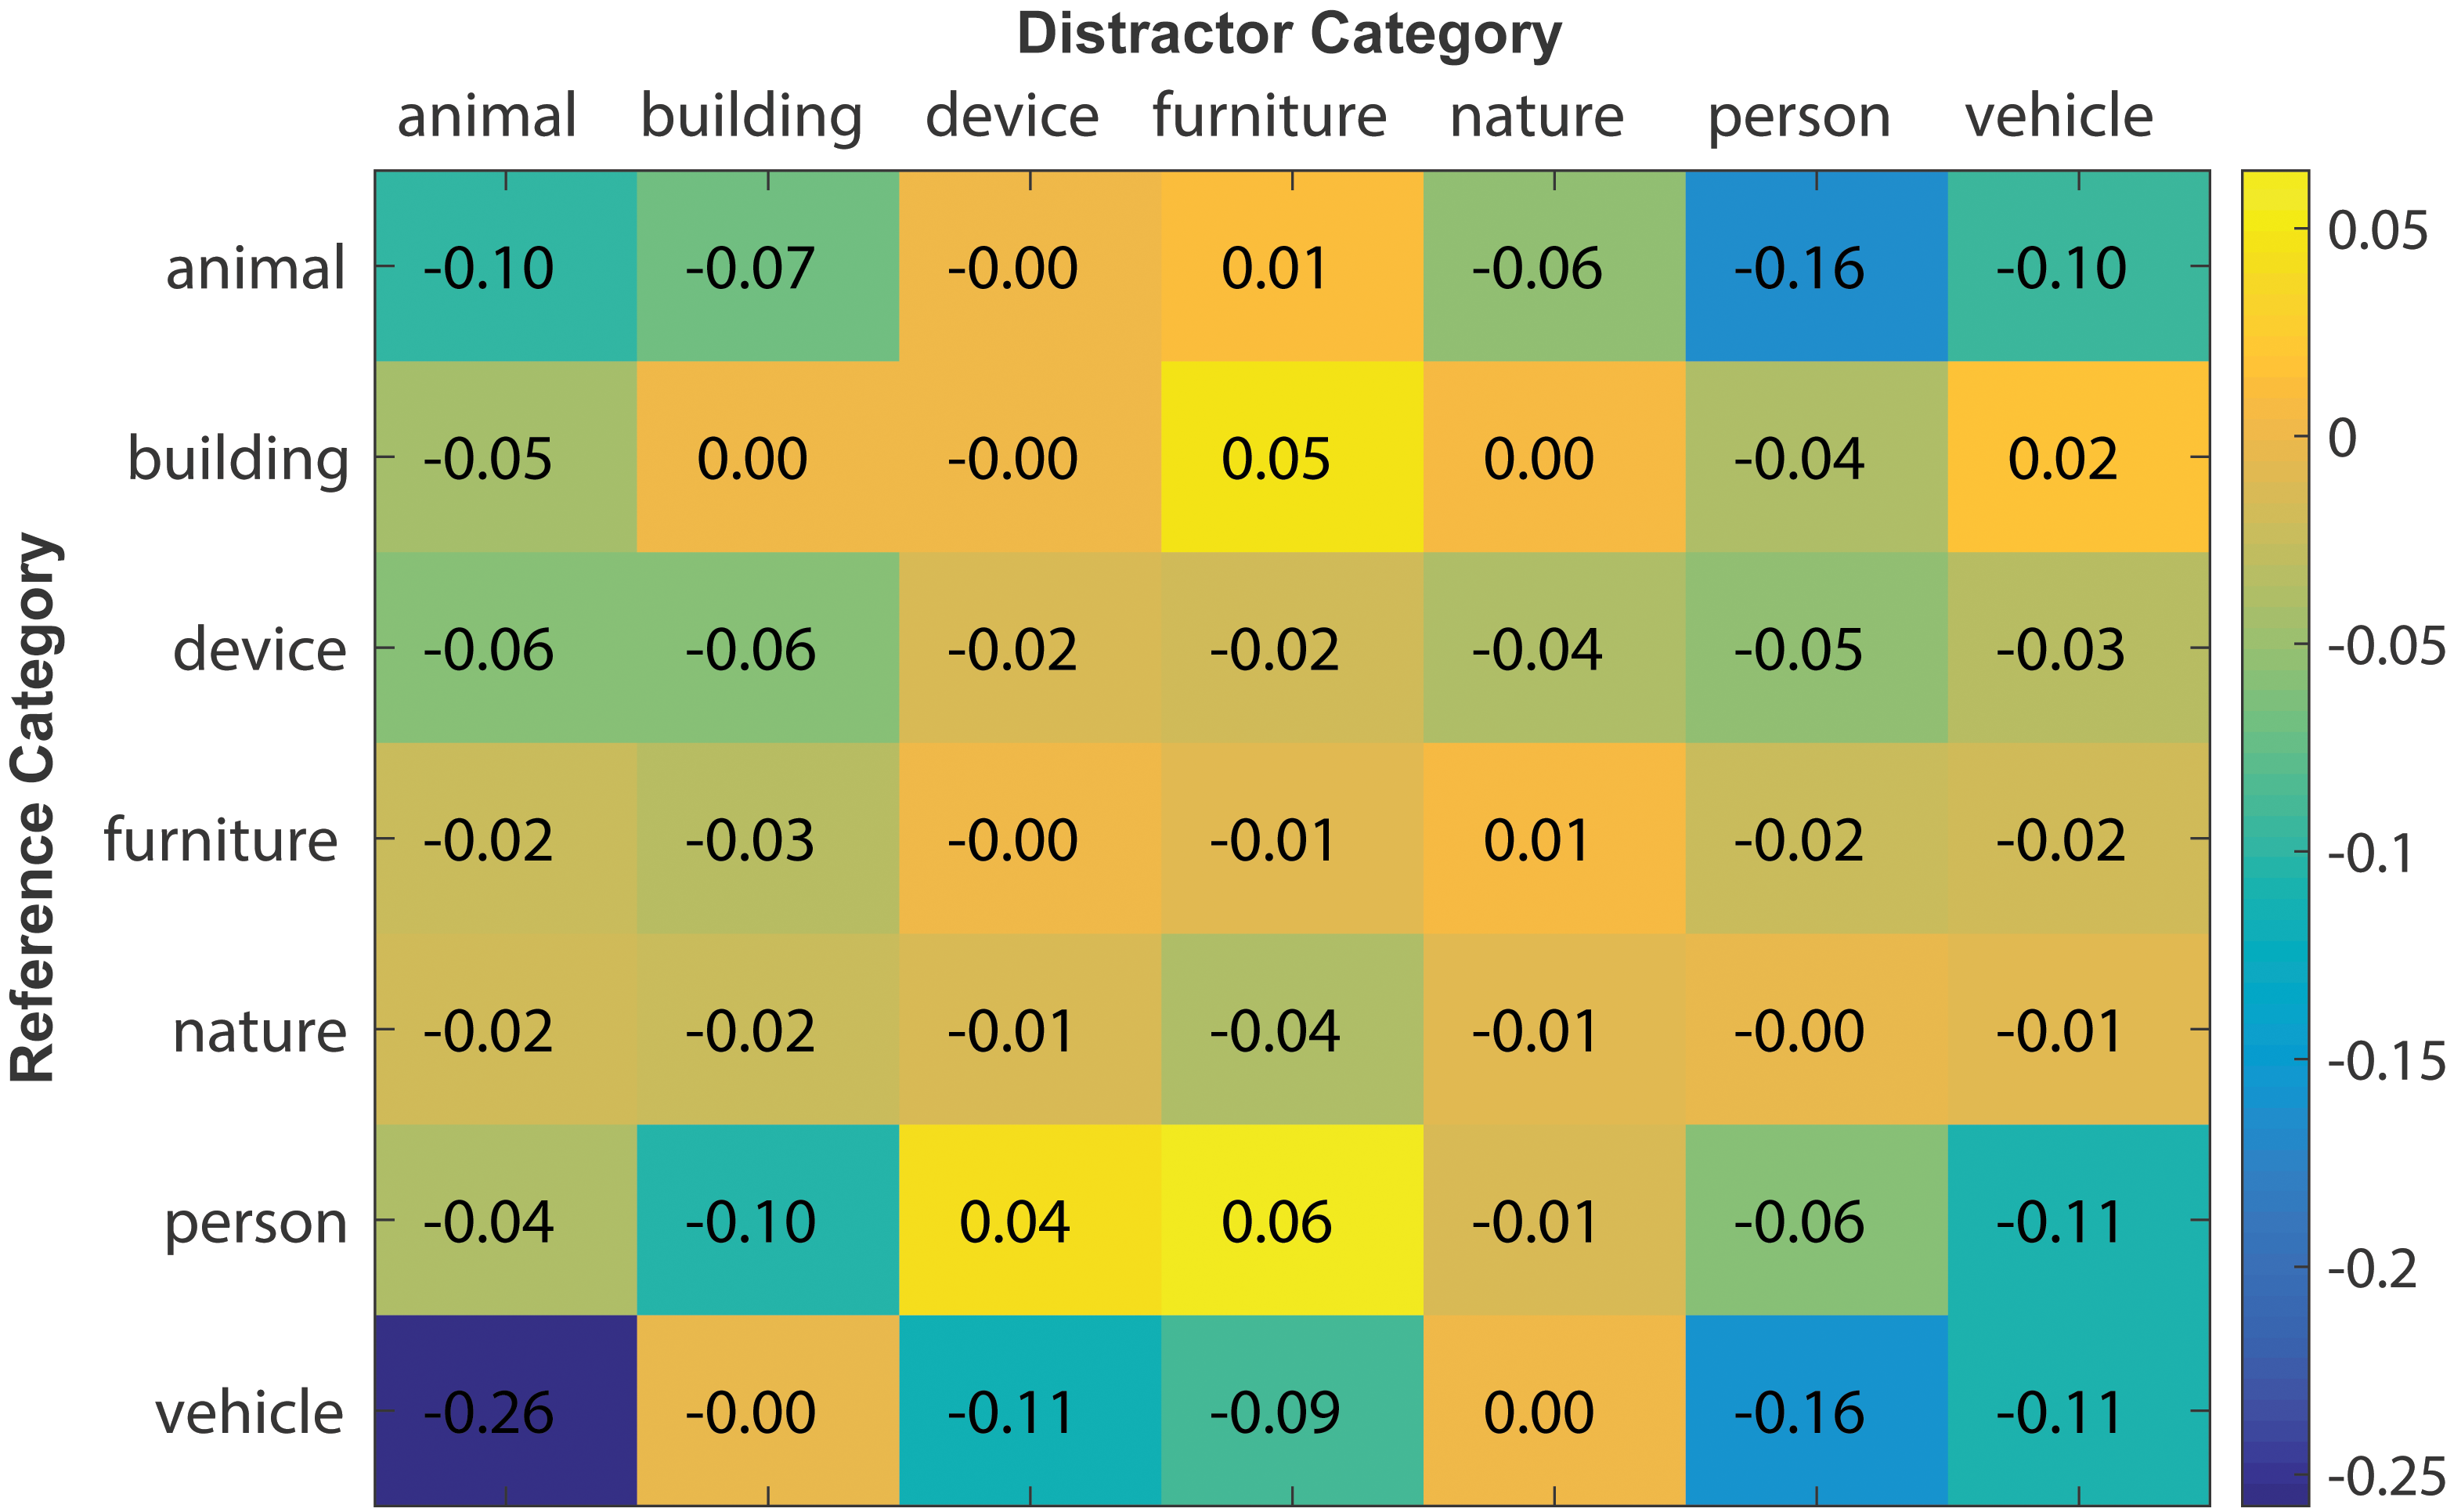
\includegraphics[width=0.47\textwidth]{figures/results/obLabel/confusionMatrix_v2.png}}
\vspace{-5mm}\caption{\footnotesize\textbf{Inter-class object memorability relationship.} The effect on memorability a distractor category has on each reference category }\label{fig:obLabelPair}
\end{figure}

\vspace{3pt}\noindent\textbf{Inter-class memorability:} How much is the memorability of a particular object category affected when it co-occurs with another object category (or another instance of the same category)? To quantify the effect of one category on another, we consider each pairwise combination of categories and gather all images that contain at least one object from both categories. By taking one category as the \emph{reference} and the other as the \emph{distractor}, we compute the average memorability score $m_{R|D}$ of the reference in the  images common to the reference and distractor. To isolate the effect of the distractor, we compute the memorability difference $\Delta m=(m_{R|D}-m_R)$, where $m_R$ is the memorability score of the reference in all images where it exists. Figure \ref{fig:obLabelPair} shows $\Delta m$ for all possible reference and distractor pairs. It is clear that  $\Delta m$ for low-memorability categories (i.e. nature, furniture, device, and building) is not significantly affected by the presence of other categories. %Instead, their memorability tends to remain low across all contexts.



Also, the memorability of the animal category maintains its high score in the presence of other categories, except vehicles, people, and itself, where it decreases substantially. The memorability of people tends to be unaffected by the presence of most other categories including itself. However, it decreases in the presence of vehicles and buildings. This could be due to the fact that people in images containing vehicles or buildings are usually zoomed out and smaller in size (refer to Figure \ref{fig:qualInterClass}). The memorability of the vehicle category is strongly affected by the presence of other object categories. In particular, it drops significantly in the presence of another vehicle, people, and animals.


\begin{figure}[t]
\centering
\subfigure{\centering \includegraphics[height = 1.1 cm]{figures/results/obLabel/inter-class/14.jpg}}
\subfigure{\centering \includegraphics[height = 1.1 cm]{figures/results/obLabel/inter-class/85.jpg}}
\subfigure{\centering \includegraphics[height = 1.1 cm]{figures/results/obLabel/inter-class/10.jpg}}
\subfigure{\centering \includegraphics[height = 1.1 cm]{figures/results/obLabel/inter-class/128.jpg}}
\subfigure{\centering \includegraphics[height = 1.1 cm]{figures/results/obLabel/inter-class/102.jpg}}
\subfigure{\centering \includegraphics[height = 1.1 cm]{figures/results/obLabel/inter-class/129.jpg}}\\
\vspace{-2mm}
\subfigure{\centering \includegraphics[height = 1.1 cm]{figures/results/obLabel/inter-class/14.png}}
\subfigure{\centering \includegraphics[height = 1.1 cm]{figures/results/obLabel/inter-class/85.png}}
\subfigure{\centering \includegraphics[height = 1.1 cm]{figures/results/obLabel/inter-class/10.png}}
\subfigure{\centering \includegraphics[height = 1.1 cm]{figures/results/obLabel/inter-class/128.png}}
\subfigure{\centering \includegraphics[height = 1.1 cm]{figures/results/obLabel/inter-class/102.png}}
\subfigure{\centering \includegraphics[height = 1.1 cm]{figures/results/obLabel/inter-class/129.png}}
\vspace{-5mm}\caption{\footnotesize\textbf{Memorability of person in presence of other categories.} Top row: Images where a person co-occurs with other categories. Bottom row: Ground truth object memorability maps. In the presence of buildings, the memorability of person can drop. In the presence of a vehicle or animal, the person usually is more memorable. }\label{fig:qualInterClass}
\end{figure}

In summary, when an animal, vehicle or a person co-occur in the same image, the memorability of all three categories usually decreases. However, this pattern of change in memorability is category-specific in general. For example, when a vehicle and animal are present in the same image, the animal is generally more memorable, even though both their memorability scores drop significantly. When a vehicle or an animal co-occurs with a person, the person is generally more memorable (also shown in Figure \ref{fig:qualInterClass}).









\subsection{How are object \& image memorability related?}

\begin{figure*}[!thb]
\centering
\subfigure{\centering \includegraphics[width=1\textwidth]{figures/results/imMem/qual.png}}
\vspace{-16pt}\caption{\footnotesize\textbf{Max object memorability predicts image memorability.} Top row: most memorable images taken from our dataset along with their highest memorable object and their respective memorability scores. Bottom row: least memorable images in the dataset along with their most memorable object and their respective memorability scores. We notice that the maximum object memorability correlates strongly with image memorability in both the cases. }\label{fig:imMemQual}%\vspace{-12pt}
\end{figure*}

Until now, we have studied what objects people remember and the factors that influence their memorability, but to what extent does the memorability of individual objects affect the overall memorability of an image? Moreover, if an image is highly memorable, what can we say about the memorability of the objects inside those images (and vice versa)? To shed light on these queries, we conducted a second large-scale experiment on Amazon Mechanical Turk for all images in our dataset to gather their respective \emph{image} memorability scores. For this experiment, we followed the same strategy as the memory game experiment proposed in \cite{isola11}. A series of images from our dataset and Microsoft COCO dataset \cite{coco14} (i.e. `filler' images) were flashed for $1$ second each, and subjects were instructed to press a key whenever they detected a repeat presentation of an image. A total of $350$ workers participated in this experiment with each image being viewed $80$ times on average. The rank correlation after averaging over $25$ random splits was $0.7$, thus, validating annotator consistency in  the image memorability scores.






Using results from the previous experiments, we computed the correlation between the scores of the single most memorable \emph{object} in each image and the memorability score of each \emph{image}. This correlation is moderately high with $\rho=0.4$, suggesting that the most memorable object in an  image plays a crucial role in determining the overall memorability of an image. To investigate this finding in relation to some extreme cases, we repeated the same analysis as above but on a subset of the data containing the $100$ most memorable images and the $100$ least memorable images. The correlation between maximum object memorability and image memorability for this subset of images increased significantly to $\rho=0.62$. This means that maximum object memorability serves as a strong indicator of whether an image is \textit{highly} memorable or \emph{not} memorable at all. In other words, images that are highly memorable contain at least one highly memorable object and images with low memorability usually do not contain a single highly memorable object (refer to Figure \ref{fig:imMemQual}).

It seems that maximum object memorability is highly explanatory, but does this behavior generalize across object categories? We further computed the correlation between maximum object and image memorability for each individual object category. The correlation for the categories were: animal ($\rho=0.38$), building ($\rho=0.22$), device ($\rho=0.47$), furniture ($\rho=0.53$), nature ($\rho=0.64$), person ($\rho=0.54$), and vehicle ($\rho=0.30$) which shows that certain categories are more strongly correlated than others. For example, images containing animals, buildings, or vehicles as the most memorable objects tend to have varying degree of image memorability (indicated by their lower $\rho$ values). On the other hand, device, furniture, nature, and person are strongly correlated with image memorability, indicating that if an image's most memorable object belongs to one of these categories, the object memorability score is strongly predictive of the image memorability score. We can imagine scenarios in which this information is potentially useful. For example, in vision systems that are tasked to predict scene memorability, a \textit{single} object and its category can serve as a strong prior in predicting this score.







